% Sweave("u:/R230/samroc-ex.Rnw", echo = TRUE)
%\VignetteIndexEntry{samroc - example}
%\VignetteDepends{SAGx,multtest, hu6800}
%\VignetteKeywords{Expression Analysis}
%\VignettePackage{SAGx}

\documentclass[11pt]{article}
\usepackage{geometry}\usepackage{color}

\definecolor{darkblue}{rgb}{0.0,0.0,0.75}
\usepackage[%
baseurl={http://www.bioconductor.org},%
pdftitle={Samroc example},%
pdfauthor={Per Broberg},%
pdfsubject={SAGx},%
pdfkeywords={Bioconductor},%
pagebackref,bookmarks,colorlinks,linkcolor=darkblue,citecolor=darkblue,%
pagecolor=darkblue,raiselinks,plainpages,pdftex]{hyperref}


%------------------------------------------------------------
% newcommand
%------------------------------------------------------------
\newcommand{\arsinh}{\mathop{\mathgroup\symoperators arsinh}\nolimits}
\newcommand{\Robject}[1]{\texttt{#1}}
\newcommand{\Rpackage}[1]{\textit{#1}}
\newcommand{\Rclass}[1]{\textit{#1}}
\newcommand{\Rfunction}[1]{{\small\texttt{#1}}}

\newcommand{\myincfig}[3]{%
  \begin{figure}[htbp]
    \begin{center}
      \includegraphics[width=#2]{#1}
      \caption{\label{#1}#3}
    \end{center}
  \end{figure}
}

\usepackage[authoryear,round]{natbib}
\usepackage{graphicx}
\usepackage{amsfonts}


\usepackage{//SELUDSFS01VS1/pbg$/R/R-2.3.0/share/texmf/Sweave}
\begin{document}

%------------------------------------------------------------
\title{Samroc example}
%------------------------------------------------------------
\author{Per Broberg}
\maketitle


\section*{Analysis of the data from Golub \textit{et al.}}

Consider the microarray experiment in \cite{golubetal} where ALL and AML subtypes of leukemia are compared.
The data are available within package \Rpackage{multtest}. 

We can analyse those data in \Rpackage{SAGx}  with the function \textit{samrocNboot}. The ideas behind
it are presented in \cite{broberg:2003}. Briefly, the method relies on a penalised \textit{t}-test statistica $ d = (\bar{x}_1 - \bar{x}_2)/(S + a)$ 
with fudge factor $a$ \cite{efron:2001}. In this case the effect estimated consists of a difference in group means. In general 
the method can estimate and test one such effect in the presence of explanatory variables such as AGE or GENDER using a linear model. In such a case
the function \Rfunction{samrocN} provides a solution. Example code now follows. 

\begin{Schunk}
\begin{Sinput}
> library(multtest)
> data(golub)
> set.seed(849867)
> samroc.res <- samrocNboot(data = golub, formula = ~as.factor(golub.cl))
> show(samroc.res)
\end{Sinput}
\begin{Soutput}
Samroc result:
Data: 38 samples with 3051 genes.
Model: ~ as.factor(golub.cl) 
Using 100 permutations
Fudge factor: 0.1230276 . Estimated proportion unchanged genes: 0.38 .
Annotation: Mon Jun 12 14:11:15 2006 
Call: samrocNboot golub ~as.factor(golub.cl) 
\end{Soutput}
\end{Schunk}
The function \Rfunction{samrocNboot} is used to perform a penalised \textit{t}-test. Its value is an object of class
\Rclass{samroc.result}. The functions \Rfunction{show} and \Rfunction{plot} are defined for such objects. In Figure \ref{density} the densities of the 
test statistic and its permutation null distribution are displayed. The graph was produced by invoking the \Rfunction{plot} function

\begin{Schunk}
\begin{Sinput}
> plot(samroc.res)
\end{Sinput}
\end{Schunk}


\begin{figure}[htbp]
\centering

\begin{Schunk}
\begin{Sinput}
> par(bg = "cornsilk")
> plot(samroc.res)
\end{Sinput}
\end{Schunk}
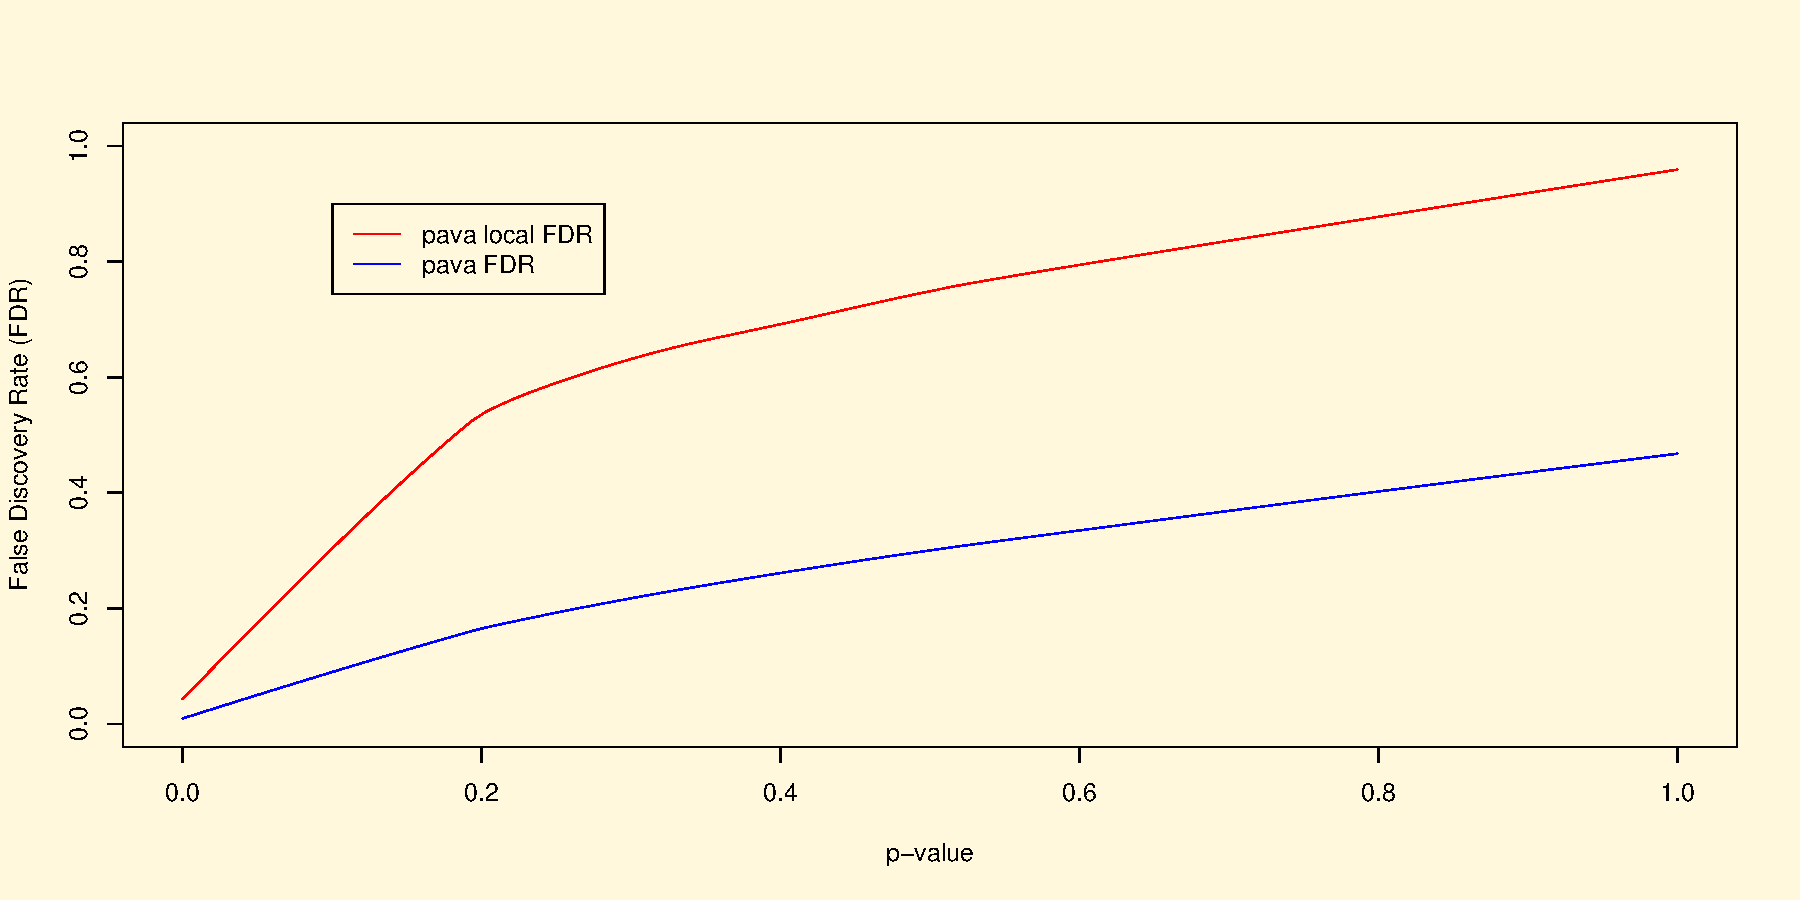
\includegraphics{samroc-ex-003}
\caption{Densities of the test statistic and of its permutation null distribution}
\label{density}
\end{figure}

\begin{figure}[htbp]
\centering

The estimated proportion unchanged genes equals 0.38. The distribution of \textit{p}-values is shown in Figure~\ref{hist1},
which confirms that many genes are changed. Furthermore, using the function \textit{pava.fdr} we obtain estimates of the FDR and 
of the local FDR, see Figure~\ref{hist2}. This function is presented in \cite{broberg:2005} and combines the local FDR estimator 
of \cite{aubert:2004} with Poisson regression (see \cite{efron:2004}) and isotonic regression.

\begin{Schunk}
\begin{Sinput}
> par(bg = "cornsilk")
> hist(samroc.res@pvalues, xlab = "p-value", main = "", col = "orange", 
+     freq = F)
> print(abline(samroc.res@p0, 0, col = "red"))
\end{Sinput}
\begin{Soutput}
NULL
\end{Soutput}
\end{Schunk}
\includegraphics{samroc-ex-004}
\caption{Histogram of the \textit{p}-values generated by function \textit{samrocNboot}}
\label{hist1}
\end{figure}

\begin{figure}[htbp]
\centering
\begin{Schunk}
\begin{Sinput}
> par(bg = "cornsilk")
> fdrs <- pava.fdr(ps = samroc.res@pvalues)
> plot(samroc.res@pvalues, fdrs$pava.local.fdr, type = "n", xlab = "p-value", 
+     ylab = "False Discovery Rate (FDR)")
> lines(lowess(samroc.res@pvalues, fdrs$pava.local.fdr), col = "red")
> lines(lowess(samroc.res@pvalues, fdrs$pava.fdr), col = "blue")
> legend(0.1, 0.9, pch = NULL, col = c("red", "blue"), c("pava local FDR", 
+     "pava FDR"), lty = 1)
\end{Sinput}
\end{Schunk}
\includegraphics{samroc-ex-005}
\caption{Scatter plot of the local false discovery rate and the false discovery rate as estimated by function \textit{pava.fdr}}
\label{hist2}
\end{figure}

One can also perform a simple Gene Set Enrichment Analysis based on the output from \Rfunction{samrocNboot} by invoking \Rfunction{GSEA.mean.t},
cf. \cite{lutian:2005} which describes a similar idea. The package \Rpackage{hu6800} maps KEGG pathways \cite{kegg:2000} onto probeset identifiers. The following code
analyses one KEGG pathway ( 00970 Aminoacyl-tRNA biosynthesis) and outputs a p-value based on the average over the pathway of 
the absolute value of the test statistic $d$.

\begin{Schunk}
\begin{Sinput}
> library(hu6800)
> kegg <- as.list(hu6800PATH2PROBE)
> probeset <- golub.gnames[, 3]
> GSEA.mean.t(data = golub, samroc = samroc.res, probeset = probeset, 
+     pway = kegg[1], absolute = TRUE, two.side = FALSE, B = 10000)
\end{Sinput}
\begin{Soutput}
    00970 
9.999e-05 
\end{Soutput}
\end{Schunk}


%%%%%%%%%%%%%%%%%%%%%%%%%%%%%%%%%%%%%%
\newpage
\bibliographystyle{plainnat}
\bibliography{samroc-ex}
%%%%%%%%%%%%%%%%%%%%%%%%%%%%%%%%%%

\end{document}
